\subsection{Verkle Tree Structure}

We use Verkle Tree to store storage data. The width of Verkle Tree is 256, and the nodes are divided into two types: InternalNode and LeafNode. We use KZG commitments for vector commitments. The order $n = 2^{251} + 17 \cdot 2^{192} + 1$ of the curve we selected is a 252-bit prime number, so we can only make safe commitments for 251-bit values. Each key consists of 32-bytes. The structure of Verkle Tree is shown in Figure \ref{fig:verkle-tree-struct}.
\begin{figure}[!ht]
    \centering
    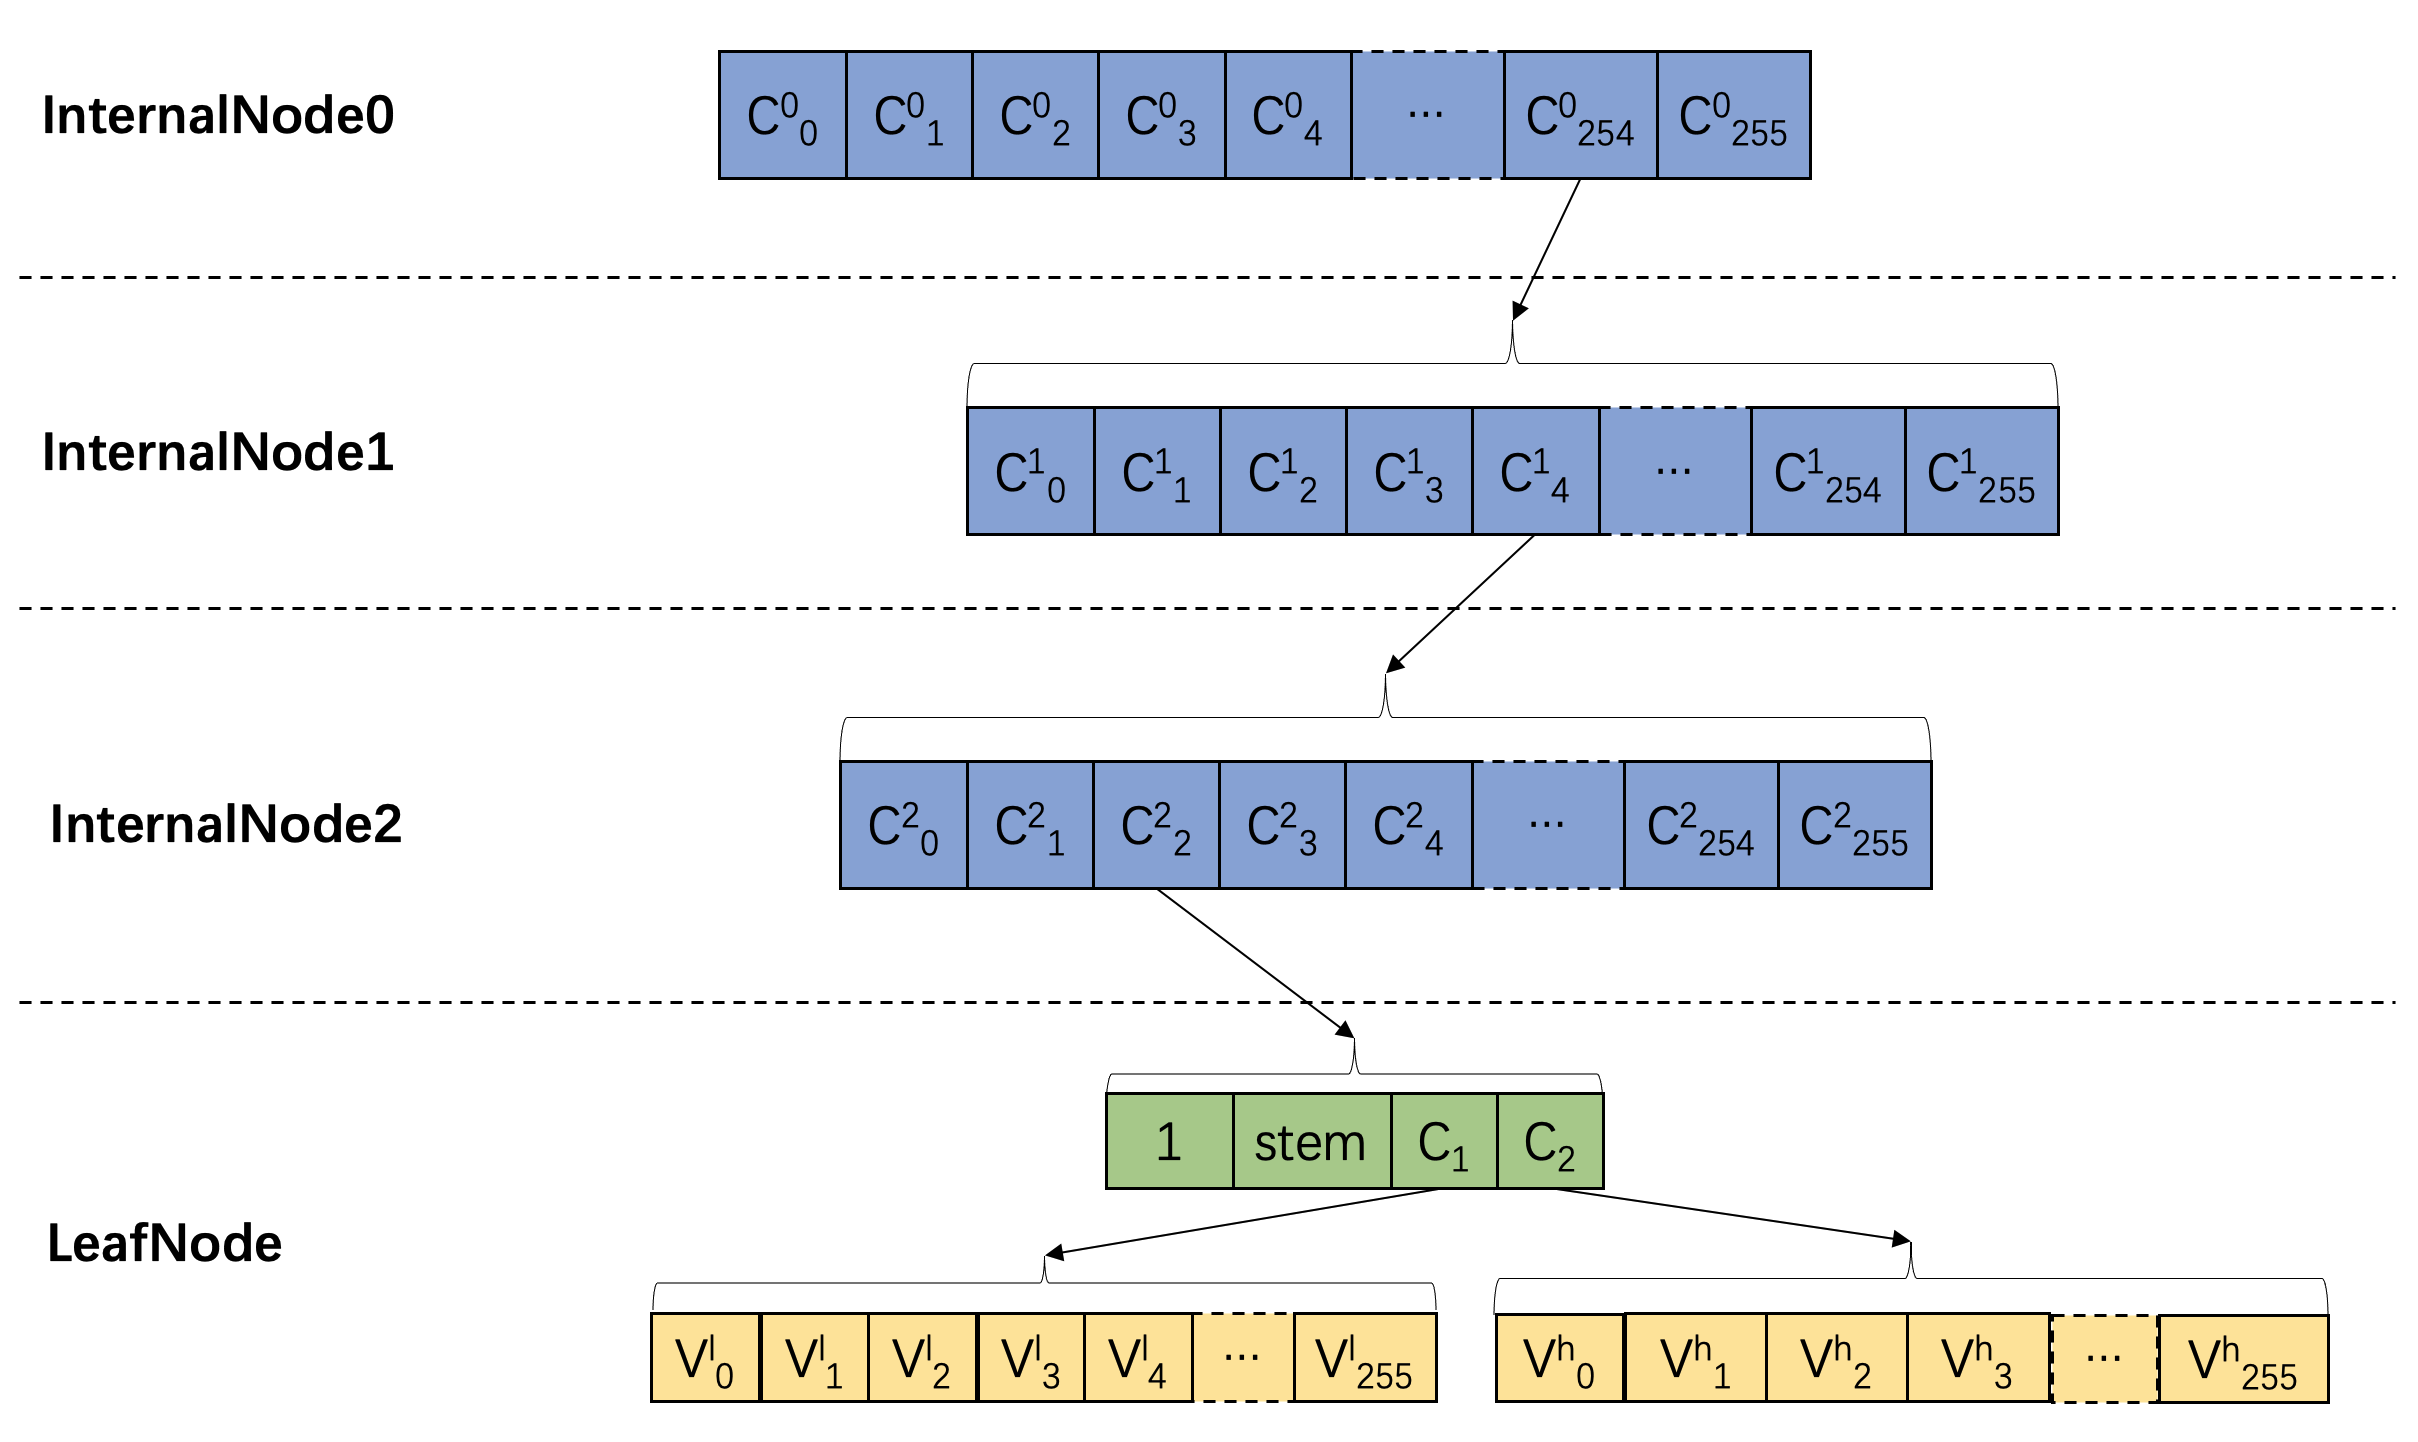
\includegraphics[width=0.8\textwidth]{storage/verkle_struct.png}
    \caption{Structure of Verkle Tree}
    \label{fig:verkle-tree-struct}
\end{figure}

For LeafNode, each value $V_i$ is 32-bytes. To make commitments to vector $\{V_i\}$, we split each value $V_i$ into two 16-byte values $V^l_i$ and $V^h_i$, and make commitments to $\{V^l_i\}$ and $\{V^h_i\}$ as $C_1 = \mathrm{Commit}(V^l_0, V^l_1, V^l_2, \ldots, V^l_{255})$, $C_2 = \mathrm{Commit}(V^h_0, V^h_1, V^h_2, \ldots, V^h_{255})$ respectively. It should especially be noted that the node will not be deleted at the data level, but use the 128th bit of $V^l_i$ as the marker bit of the deleted node. If the 128th bit of $V^l_i$ is set to 1, it means the node has been deleted. The commitment of LeafNode is composed of flag bit 1, stem and two sub-commitments $C_1$, $C_2$, i.e.
\[ C = \mathrm{Commit}(1, \mathrm{stem}, C_1, C_2). \]
The commitment to InternalNode is relatively simpler that the commitment to empty node is 0 and if the node is non-empty, just directly make commitments to all 256 commitment values, namely
\[ C = \mathrm{Commit}(C_0, C_1, C_2, \ldots, C_{255}). \]
